\section{Monidas-Plattform}
\label{mon}

Die Monidas-Plattform bildet die technische Grundlage für den Monidas Code Assist Navigator. Sie ist als IoT-Plattform konzipiert und ermöglicht die Erfassung, Verarbeitung und Überwachung von Sensordaten. Die technische Basis bilden dabei die Graphdatenbank \textit{Selva} sowie das Web-Framework \textit{Based}.

Dieses Kapitel beschreibt jene Aspekte der Monidas-Plattform, welche für die Umsetzung der in dieser Arbeit entwickelten Lösung relevant sind, um deren Kompatibilität mit der bestehenden Plattform sicherzustellen. Abschnitt~\ref{mon:plat} stellt hierzu zunächst die Entitäten vor, die für die Modellierung der Sensorüberwachung erforderlich sind. Abschnitt~\ref{abb:tech} erläutert anschliessend diejenigen Funktionalitäten und technologischen Eigenschaften von Selva und Based, auf denen die entwickelte Lösung aufbaut.

\subsection{Plattform}
\label{mon:plat}
Die Monidas-Plattform wurde in Kapitel \ref{kap:ein} im Zusammenhang mit dem Konfigurationsprozess eingeführt. Da dieser jedoch nur einen Teil der Gesamtfunktionalität abdeckt, werden in diesem Abschnitt Entitäten vorgestellt, die für die Überwachung von Sensoren relevant sind.

Zur Veranschaulichung zeigt Abbildung \ref{fig:mon_plat} die Dashboardansicht der Monidas-Plattform im Bereich „Trends“.  
Die Oberfläche listet mehrere Sensorgeräte (z.B. \textit{DatadotPilot01} bis \textit{DatadotPilot03}), die sich aktuell im Alarmzustand befinden. Für jedes Gerät werden Messdaten zur relativen Luftfeuchtigkeit und zur Temperatur der letzten 24 Stunden visualisiert – inklusive Minimal-, Maximal- und Mittelwert sowie grafischer Trendverläufe. Eine Filterleiste erlaubt die Einschränkung der Anzeige nach Gerätetyp und Status.

Die Benutzeroberfläche dient dabei lediglich der Veranschaulichung des Kontextes und ist nicht Gegenstand dieser Arbeit.  
Statt auf die grafische Oberfläche konzentriert sich diese Arbeit auf eine modellbasierte Verwaltungslogik, die direkt auf dem zugrunde liegenden Datenmodell aufbaut.  
Weitere UI-Ansichten der Monidas-Plattform werden daher im Folgenden nicht weiter berücksichtigt.

\begin{figure}[H]
  \centering
  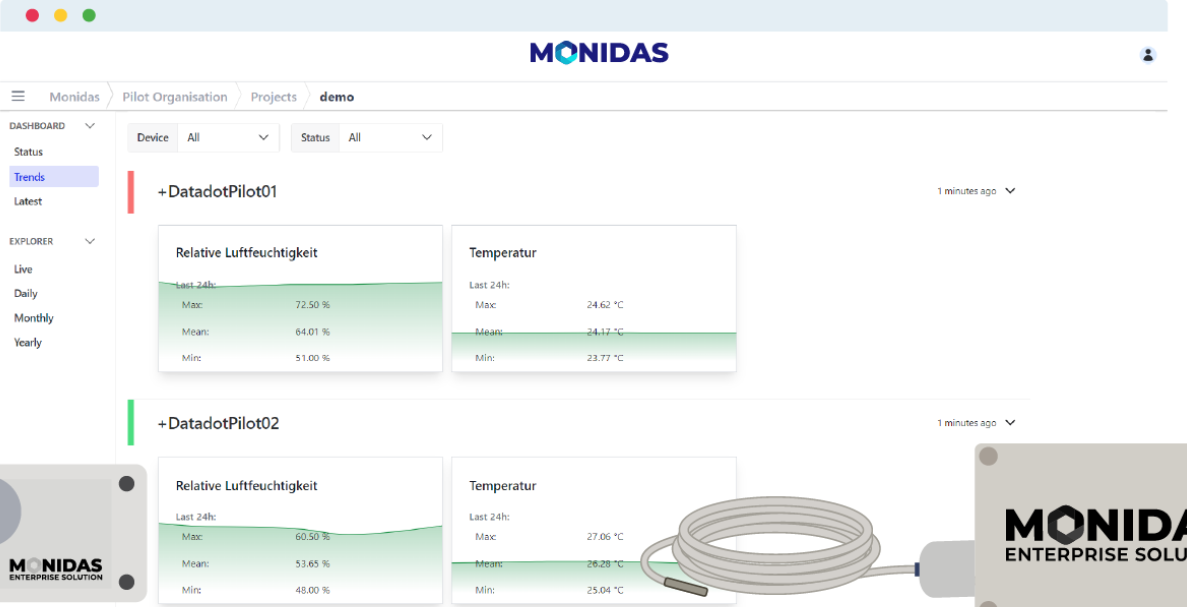
\includegraphics[width=1\linewidth]{mon_plat.png}
 \caption{Dashboardansicht mit Trendverlauf von Sensoren im Alarmzustand}
  \label{fig:mon_plat}
\end{figure}

Die dargestellte Übersicht setzt voraus, dass zuvor bestimmte Entitäten im Datenmodell der Monidas-Plattform vorhanden sind. Aufgrund der Komplexität des vollständigen Domänenmodells beschränkt sich diese Darstellung auf einen relevanten Ausschnitt. Dieser Ausschnitt wird in Abbildung \ref{fig:mon_UML} anhand eines vereinfachten UML-Diagramms veranschaulicht.

In Kapitel~\ref{kap:eva} wird das dargestellte Modell erneut aufgegriffen und hinsichtlich der Auswirkungen der entwickelten Lösung auf das bestehende System evaluiert. Dabei stehen insbesondere die Forschungsfragen zur Skalierbarkeit, Erweiterbarkeit sowie zu den architektonischen Grenzen des zugrundeliegenden Datenmodells im Mittelpunkt der Analyse.

Die folgenden Entitäten bilden die Grundlage des betrachteten Modellausschnitts:
\begin{itemize}
  \item \textbf{User}: Personen, die einer Organisation oder einem Projekt zugeordnet sind.
  \item \textbf{Organization}: Organisationen.
  \item \textbf{Project}: Projekte, die einer Organisation zugeordnet sind.
  \item \textbf{Device}: Physische Geräte (z.B. Sensoren), die Daten erfassen und übertragen.
  \item \textbf{Monitor}: Überwachungseinheiten, die Sensordaten beobachten und Aktionen auslösen.
  \item \textbf{Function}: Wertet Sensordaten aus und ermittelt daraus den Zustand des Sensors.
  \item \textbf{Template}: Vorlage, welche den Betreff und Inhalt von Benachrichtigungen definiert.
  \item \textbf{Action}: Benachrichtigt definierte Empfänger bei bestimmten Sensorereignissen.
  \item \textbf{Group}: Gruppen, die festlegen, welche Personen Benachrichtigungen erhalten.
\end{itemize}

\begin{figure}[H]
  \centering
  \includegraphics[width=1\linewidth]{mon_UML.png}
  \caption{UML-Modellausschnitt der Monidas-Plattform zur Sensorüberwachung}
  \label{fig:mon_UML}
\end{figure}

Um das Zusammenspiel der oben beschriebenen Entitäten zu verdeutlichen, folgt ein praxisnahes Beispiel:  
An der FHNW (\textit{Organization}) gibt es das Projekt \textit{Serverraum Brugg} (\textit{Project}), in dem Techniker und Administratoren (\textit{User}) tätig sind. Im Serverraum sind mehrere Temperatursensoren (\textit{Devices}) installiert, die zur Überwachung der Raumtemperatur eingesetzt werden. Ein \textit{Monitor} prüft kontinuierlich die Temperatur und nutzt eine \textit{Function}, die in JavaScript implementiert ist, um zu erkennen, ob der Wert 27°C überschreitet.  
Wird dieser Grenzwert überschritten, ändert sich der Status auf \textit{Alarm}. Dies löst eine \textit{Action} aus, die eine Benachrichtigung an die zuständige \textit{Group} sendet. Der Inhalt der Benachrichtigung basiert auf einem \textit{Template} und lautet:

\begin{quote}
  „Die Temperatur im Serverraum Brugg hat 27°C überschritten. Bitte beobachten!“
\end{quote}


\subsection{Technologien}
\label{abb:tech}
Für die Umsetzung des virtuellen Dateisystems und des Language Servers werden Technologien verwendet, die gezielt auf die bestehende Infrastruktur der Monidas-Plattform abgestimmt sind. Diese Technologien wurden in Absprache mit dem Auftraggeber ausgewählt, um eine nahtlose Integration, Wartbarkeit und Erweiterbarkeit sicherzustellen. Im Folgenden werden nur jene Aspekte beschrieben, die für das Verständnis und die Umsetzung der in dieser Arbeit entwickelten Lösung relevant sind. Es ist anzumerken, dass die verfügbare Dokumentation der eingesetzten Technologien in Form von Repository-Dokumenten vorliegt, welche grundlegende Informationen bereitstellen und nur in begrenztem Umfang detaillierte Erläuterungen enthalten.

\subsubsection*{Selva}

Als Datenbanktechnologie wird die Graphdatenbank \textit{Selva}\footnote{\url{https://github.com/atelier-saulx/selva}} eingesetzt.

\paragraph{Datenbankschema}
Selva definiert das Datenmodell mithilfe eines Datenbankschemas, das Objekttypen, deren Felder sowie die jeweils erlaubten Datentypen beschreibt. Im Rahmen dieser Arbeit werden dabei nur jene Datentypen betrachtet, die in den in Abbildung~\ref{fig:mon_UML} dargestellten Entitäten tatsächlich verwendet werden.

Zu den verwendeten einfachen Datentypen zählen \texttt{string}, \texttt{boolean} und \texttt{number}, die beispielsweise zur Speicherung von Namen, Statuswerten oder numerischen Messwerten dienen. Validierte Datentypen wie \texttt{email} stellen sicher, dass nur syntaktisch korrekte E-Mail-Adressen gespeichert werden können. Strukturierte Daten, etwa Konfigurationen innerhalb von \textit{Function}-Entitäten, werden mithilfe des Datentyps \texttt{json} gespeichert. Für die Abbildung von Beziehungen zwischen Entitäten kommen die Referenztypen \texttt{reference} und \texttt{references} zum Einsatz, die den Kardinalitäten \texttt{0..1} bzw. \texttt{0..*} entsprechen. Selva erzwingt dabei jedoch keine wechselseitigen Einschränkungen wie etwa eine verpflichtende One-to-One-Beziehung. Solche komplexeren Anforderungen müssen bei Bedarf durch die Anwendung selbst implementiert werden.



Um die korrekte Funktion und Datenintegrität des Monidas Code Assist Navigators sicherzustellen, wurden ergänzende \textit{Constraints} definiert. Diese wurden direkt im Schema ergänzt. Da Selva jedoch nur die ihr bekannten Schema-Regeln auswertet, ignoriert sie diese Erweiterungen vollständig. Die neu definierten Constraints müssen daher von der Anwendung selbst geprüft und durchgesetzt werden. Alle für den Monidas Code Assist Navigator definierten Constraints sowie deren konkrete Umsetzung werden ausführlich in Kapitel~\ref{kap:dbschema} beschrieben.

Ein vereinfachtes Beispiel eines Selva-Schemas für die in Abbildung~\ref{fig:mon_UML} gezeigten Entitäten ist in Listing~\ref{lst:schema_beispiel} dargestellt. Es zeigt, wie die Entitäten \texttt{Organization}, \texttt{Project} und \texttt{User} mit ihren jeweiligen Feldern und Beziehungen definiert werden.

\newpage


\lstinputlisting[
  caption={Beispiel eines Selva-Datenbankschemas}, 
  label={lst:schema_beispiel},
  style=customtypescript
]{listings/schema_bsp.json}


\paragraph{Datenzugriff}
\label{sec:Datenzugriff}Um auf die im Schema definierten Objekte zugreifen und diese manipulieren zu können, stellt Selva eine API mit grundlegenden Operationen bereit. Mithilfe dieser API lassen sich Objekte erstellen und aktualisieren (\texttt{set}), abfragen (\texttt{get}), löschen (\texttt{delete}) sowie in Echtzeit überwachen (\texttt{observe}). Die konkrete Formulierung dieser Operationen erfolgt über eine eigene Query DSL, die auf JavaScript-Objekten basiert. Ähnlich wie beispielsweise bei GraphQL werden dabei die gewünschten Felder und Beziehungen präzise über eine strukturierte Objektdefinition angegeben.

In Selva existieren mehrere intern vordefinierte Felder, die nicht explizit im Schema definiert werden müssen. Im Rahmen dieser Arbeit sind die Felder \textit{ID} und \textit{Aliases} relevant. Die ID dient der eindeutigen Identifikation eines jeden Objekts und wird entweder durch Selva generiert oder manuell vorgegeben. Wird keine ID angegeben, erzeugt die Datenbank eine neue ID. In diesem Fall muss zwingend der Typ des Objekts (z.B. \texttt{Organization}) angegeben werden. Zudem bietet Selva die Möglichkeit, deterministisch immer dieselbe ID zu erzeugen. Zusätzlich zur ID besitzen alle Objekte Aliases. Ein Objekt kann mehrere Aliases besitzen, und es ist möglich, dass verschiedene Objekte denselben Alias verwenden. Ihre genaue Bedeutung und Verwendung hängt von der jeweiligen Anwendungslogik ab. Grundsätzlich dienen Aliases dazu, Datenobjekte benutzerfreundlicher und flexibler abzurufen oder zu referenzieren.

Listing~\ref{lst:selva_bsp} veranschaulicht die beschriebenen Operationen in einem praxisnahen Anwendungsfall. Zunächst wird eine neue Organisation mit einem Alias erstellt. Danach wird diese sowohl über die automatisch generierte ID als auch über den definierten Alias abgefragt. Anschliessend demonstriert das Beispiel die Überwachung von Echtzeitänderungen am Objekt. Abschliessend wird gezeigt, wie mithilfe eines externen Alias eine eindeutige ID generiert werden kann, um gezielt ein weiteres Objekt zu erstellen und dieses anschliessend zu löschen. Die in diesem Beispiel dargestellten Operationen bilden die Basis für die entwickelte Lösung, insbesondere für die Umsetzung des virtuellen Filesystems und des Language Servers.

\newpage


\lstinputlisting[
  caption={Beispiel zur Verwendung der Selva-API}, 
  label={lst:selva_bsp},
  style=customtypescript
]{listings/selva_bsp.js}

\subsubsection*{Based}
PLS HELP Muesii das überhaupt ihfüre wenni es eig nie erwähnt ?

Selva kanni jo lo welli aliases usw verwänd unds Schema oder ?